% GNUPLOT: LaTeX picture with Postscript
\begingroup
  % Encoding inside the plot.  In the header of your document, this encoding
  % should to defined, e.g., by using
  % \usepackage[latin1,<other encodings>]{inputenc}
  \inputencoding{latin1}%
  \makeatletter
  \providecommand\color[2][]{%
    \GenericError{(gnuplot) \space\space\space\@spaces}{%
      Package color not loaded in conjunction with
      terminal option `colourtext'%
    }{See the gnuplot documentation for explanation.%
    }{Either use 'blacktext' in gnuplot or load the package
      color.sty in LaTeX.}%
    \renewcommand\color[2][]{}%
  }%
  \providecommand\includegraphics[2][]{%
    \GenericError{(gnuplot) \space\space\space\@spaces}{%
      Package graphicx or graphics not loaded%
    }{See the gnuplot documentation for explanation.%
    }{The gnuplot epslatex terminal needs graphicx.sty or graphics.sty.}%
    \renewcommand\includegraphics[2][]{}%
  }%
  \providecommand\rotatebox[2]{#2}%
  \@ifundefined{ifGPcolor}{%
    \newif\ifGPcolor
    \GPcolortrue
  }{}%
  \@ifundefined{ifGPblacktext}{%
    \newif\ifGPblacktext
    \GPblacktexttrue
  }{}%
  % define a \g@addto@macro without @ in the name:
  \let\gplgaddtomacro\g@addto@macro
  % define empty templates for all commands taking text:
  \gdef\gplbacktext{}%
  \gdef\gplfronttext{}%
  \makeatother
  \ifGPblacktext
    % no textcolor at all
    \def\colorrgb#1{}%
    \def\colorgray#1{}%
  \else
    % gray or color?
    \ifGPcolor
      \def\colorrgb#1{\color[rgb]{#1}}%
      \def\colorgray#1{\color[gray]{#1}}%
      \expandafter\def\csname LTw\endcsname{\color{white}}%
      \expandafter\def\csname LTb\endcsname{\color{black}}%
      \expandafter\def\csname LTa\endcsname{\color{black}}%
      \expandafter\def\csname LT0\endcsname{\color[rgb]{1,0,0}}%
      \expandafter\def\csname LT1\endcsname{\color[rgb]{0,1,0}}%
      \expandafter\def\csname LT2\endcsname{\color[rgb]{0,0,1}}%
      \expandafter\def\csname LT3\endcsname{\color[rgb]{1,0,1}}%
      \expandafter\def\csname LT4\endcsname{\color[rgb]{0,1,1}}%
      \expandafter\def\csname LT5\endcsname{\color[rgb]{1,1,0}}%
      \expandafter\def\csname LT6\endcsname{\color[rgb]{0,0,0}}%
      \expandafter\def\csname LT7\endcsname{\color[rgb]{1,0.3,0}}%
      \expandafter\def\csname LT8\endcsname{\color[rgb]{0.5,0.5,0.5}}%
    \else
      % gray
      \def\colorrgb#1{\color{black}}%
      \def\colorgray#1{\color[gray]{#1}}%
      \expandafter\def\csname LTw\endcsname{\color{white}}%
      \expandafter\def\csname LTb\endcsname{\color{black}}%
      \expandafter\def\csname LTa\endcsname{\color{black}}%
      \expandafter\def\csname LT0\endcsname{\color{black}}%
      \expandafter\def\csname LT1\endcsname{\color{black}}%
      \expandafter\def\csname LT2\endcsname{\color{black}}%
      \expandafter\def\csname LT3\endcsname{\color{black}}%
      \expandafter\def\csname LT4\endcsname{\color{black}}%
      \expandafter\def\csname LT5\endcsname{\color{black}}%
      \expandafter\def\csname LT6\endcsname{\color{black}}%
      \expandafter\def\csname LT7\endcsname{\color{black}}%
      \expandafter\def\csname LT8\endcsname{\color{black}}%
    \fi
  \fi
    \setlength{\unitlength}{0.0500bp}%
    \ifx\gptboxheight\undefined%
      \newlength{\gptboxheight}%
      \newlength{\gptboxwidth}%
      \newsavebox{\gptboxtext}%
    \fi%
    \setlength{\fboxrule}{0.5pt}%
    \setlength{\fboxsep}{1pt}%
\begin{picture}(7200.00,4320.00)%
    \gplgaddtomacro\gplbacktext{%
      \colorrgb{0.00,0.00,0.00}%%
      \put(1998,965){\makebox(0,0)[r]{\strut{}$1.5$}}%
      \colorrgb{0.00,0.00,0.00}%%
      \put(1998,1591){\makebox(0,0)[r]{\strut{}$2$}}%
      \colorrgb{0.00,0.00,0.00}%%
      \put(1998,2217){\makebox(0,0)[r]{\strut{}$2.5$}}%
      \colorrgb{0.00,0.00,0.00}%%
      \put(1998,2843){\makebox(0,0)[r]{\strut{}$3$}}%
      \colorrgb{0.00,0.00,0.00}%%
      \put(1998,3469){\makebox(0,0)[r]{\strut{}$3.5$}}%
      \colorrgb{0.00,0.00,0.00}%%
      \put(1998,4095){\makebox(0,0)[r]{\strut{}$4$}}%
      \colorrgb{0.00,0.00,0.00}%%
      \put(2423,448){\makebox(0,0){\strut{}$1.5$}}%
      \colorrgb{0.00,0.00,0.00}%%
      \put(3049,448){\makebox(0,0){\strut{}$2$}}%
      \colorrgb{0.00,0.00,0.00}%%
      \put(3675,448){\makebox(0,0){\strut{}$2.5$}}%
      \colorrgb{0.00,0.00,0.00}%%
      \put(4301,448){\makebox(0,0){\strut{}$3$}}%
      \colorrgb{0.00,0.00,0.00}%%
      \put(4927,448){\makebox(0,0){\strut{}$3.5$}}%
      \colorrgb{0.00,0.00,0.00}%%
      \put(5553,448){\makebox(0,0){\strut{}$4$}}%
    }%
    \gplgaddtomacro\gplfronttext{%
      \csname LTb\endcsname%%
      \put(1476,2373){\rotatebox{-270}{\makebox(0,0){\strut{}R_{NC_2}, {\305}}}}%
      \csname LTb\endcsname%%
      \put(3831,142){\makebox(0,0){\strut{}R_{NC_1}, {\305}}}%
      \csname LTb\endcsname%%
      \settowidth{\gptboxwidth}{\widthof{0}}
	\advance\gptboxwidth by 2\fboxsep
      \savebox{\gptboxtext}{\parbox[c][\totalheight+2\fboxsep]{\gptboxwidth}{\centering{0}}}
        \definecolor{tbcol}{rgb}{1,1,1}
	\put(2554,777){\makebox(0,0){\colorbox{tbcol}{\usebox{\gptboxtext}}}}
      \csname LTb\endcsname%%
      \csname LTb\endcsname%%
      \settowidth{\gptboxwidth}{\widthof{0}}
	\advance\gptboxwidth by 2\fboxsep
      \savebox{\gptboxtext}{\parbox[c][\totalheight+2\fboxsep]{\gptboxwidth}{\centering{0}}}
        \definecolor{tbcol}{rgb}{1,1,1}
	\put(2585,1028){\makebox(0,0){\colorbox{tbcol}{\usebox{\gptboxtext}}}}
      \csname LTb\endcsname%%
      \csname LTb\endcsname%%
      \settowidth{\gptboxwidth}{\widthof{-0.1}}
	\advance\gptboxwidth by 2\fboxsep
      \savebox{\gptboxtext}{\parbox[c][\totalheight+2\fboxsep]{\gptboxwidth}{\centering{-0.1}}}
        \definecolor{tbcol}{rgb}{1,1,1}
	\put(3074,652){\makebox(0,0){\colorbox{tbcol}{\usebox{\gptboxtext}}}}
      \csname LTb\endcsname%%
      \csname LTb\endcsname%%
      \settowidth{\gptboxwidth}{\widthof{-0.1}}
	\advance\gptboxwidth by 2\fboxsep
      \savebox{\gptboxtext}{\parbox[c][\totalheight+2\fboxsep]{\gptboxwidth}{\centering{-0.1}}}
        \definecolor{tbcol}{rgb}{1,1,1}
	\put(2736,1568){\makebox(0,0){\colorbox{tbcol}{\usebox{\gptboxtext}}}}
      \csname LTb\endcsname%%
      \csname LTb\endcsname%%
      \settowidth{\gptboxwidth}{\widthof{-0.2}}
	\advance\gptboxwidth by 2\fboxsep
      \savebox{\gptboxtext}{\parbox[c][\totalheight+2\fboxsep]{\gptboxwidth}{\centering{-0.2}}}
        \definecolor{tbcol}{rgb}{1,1,1}
	\put(3409,652){\makebox(0,0){\colorbox{tbcol}{\usebox{\gptboxtext}}}}
      \csname LTb\endcsname%%
      \csname LTb\endcsname%%
      \settowidth{\gptboxwidth}{\widthof{-0.2}}
	\advance\gptboxwidth by 2\fboxsep
      \savebox{\gptboxtext}{\parbox[c][\totalheight+2\fboxsep]{\gptboxwidth}{\centering{-0.2}}}
        \definecolor{tbcol}{rgb}{1,1,1}
	\put(3112,1604){\makebox(0,0){\colorbox{tbcol}{\usebox{\gptboxtext}}}}
      \csname LTb\endcsname%%
      \csname LTb\endcsname%%
      \settowidth{\gptboxwidth}{\widthof{-0.2}}
	\advance\gptboxwidth by 2\fboxsep
      \savebox{\gptboxtext}{\parbox[c][\totalheight+2\fboxsep]{\gptboxwidth}{\centering{-0.2}}}
        \definecolor{tbcol}{rgb}{1,1,1}
	\put(2173,1951){\makebox(0,0){\colorbox{tbcol}{\usebox{\gptboxtext}}}}
      \csname LTb\endcsname%%
      \csname LTb\endcsname%%
      \settowidth{\gptboxwidth}{\widthof{-0.3}}
	\advance\gptboxwidth by 2\fboxsep
      \savebox{\gptboxtext}{\parbox[c][\totalheight+2\fboxsep]{\gptboxwidth}{\centering{-0.3}}}
        \definecolor{tbcol}{rgb}{1,1,1}
	\put(3857,652){\makebox(0,0){\colorbox{tbcol}{\usebox{\gptboxtext}}}}
      \csname LTb\endcsname%%
      \csname LTb\endcsname%%
      \settowidth{\gptboxwidth}{\widthof{-0.3}}
	\advance\gptboxwidth by 2\fboxsep
      \savebox{\gptboxtext}{\parbox[c][\totalheight+2\fboxsep]{\gptboxwidth}{\centering{-0.3}}}
        \definecolor{tbcol}{rgb}{1,1,1}
	\put(3498,1591){\makebox(0,0){\colorbox{tbcol}{\usebox{\gptboxtext}}}}
      \csname LTb\endcsname%%
      \csname LTb\endcsname%%
      \settowidth{\gptboxwidth}{\widthof{-0.3}}
	\advance\gptboxwidth by 2\fboxsep
      \savebox{\gptboxtext}{\parbox[c][\totalheight+2\fboxsep]{\gptboxwidth}{\centering{-0.3}}}
        \definecolor{tbcol}{rgb}{1,1,1}
	\put(2866,2217){\makebox(0,0){\colorbox{tbcol}{\usebox{\gptboxtext}}}}
      \csname LTb\endcsname%%
      \csname LTb\endcsname%%
      \settowidth{\gptboxwidth}{\widthof{-0.4}}
	\advance\gptboxwidth by 2\fboxsep
      \savebox{\gptboxtext}{\parbox[c][\totalheight+2\fboxsep]{\gptboxwidth}{\centering{-0.4}}}
        \definecolor{tbcol}{rgb}{1,1,1}
	\put(5553,1495){\makebox(0,0){\colorbox{tbcol}{\usebox{\gptboxtext}}}}
      \csname LTb\endcsname%%
      \csname LTb\endcsname%%
      \settowidth{\gptboxwidth}{\widthof{-0.4}}
	\advance\gptboxwidth by 2\fboxsep
      \savebox{\gptboxtext}{\parbox[c][\totalheight+2\fboxsep]{\gptboxwidth}{\centering{-0.4}}}
        \definecolor{tbcol}{rgb}{1,1,1}
	\put(3612,1939){\makebox(0,0){\colorbox{tbcol}{\usebox{\gptboxtext}}}}
      \csname LTb\endcsname%%
      \csname LTb\endcsname%%
      \settowidth{\gptboxwidth}{\widthof{-0.4}}
	\advance\gptboxwidth by 2\fboxsep
      \savebox{\gptboxtext}{\parbox[c][\totalheight+2\fboxsep]{\gptboxwidth}{\centering{-0.4}}}
        \definecolor{tbcol}{rgb}{1,1,1}
	\put(3014,2843){\makebox(0,0){\colorbox{tbcol}{\usebox{\gptboxtext}}}}
      \csname LTb\endcsname%%
      \csname LTb\endcsname%%
      \settowidth{\gptboxwidth}{\widthof{-0.5}}
	\advance\gptboxwidth by 2\fboxsep
      \savebox{\gptboxtext}{\parbox[c][\totalheight+2\fboxsep]{\gptboxwidth}{\centering{-0.5}}}
        \definecolor{tbcol}{rgb}{1,1,1}
	\put(5553,2126){\makebox(0,0){\colorbox{tbcol}{\usebox{\gptboxtext}}}}
      \csname LTb\endcsname%%
      \csname LTb\endcsname%%
      \settowidth{\gptboxwidth}{\widthof{-0.5}}
	\advance\gptboxwidth by 2\fboxsep
      \savebox{\gptboxtext}{\parbox[c][\totalheight+2\fboxsep]{\gptboxwidth}{\centering{-0.5}}}
        \definecolor{tbcol}{rgb}{1,1,1}
	\put(3648,2843){\makebox(0,0){\colorbox{tbcol}{\usebox{\gptboxtext}}}}
      \csname LTb\endcsname%%
    }%
    \gplbacktext
    \put(0,0){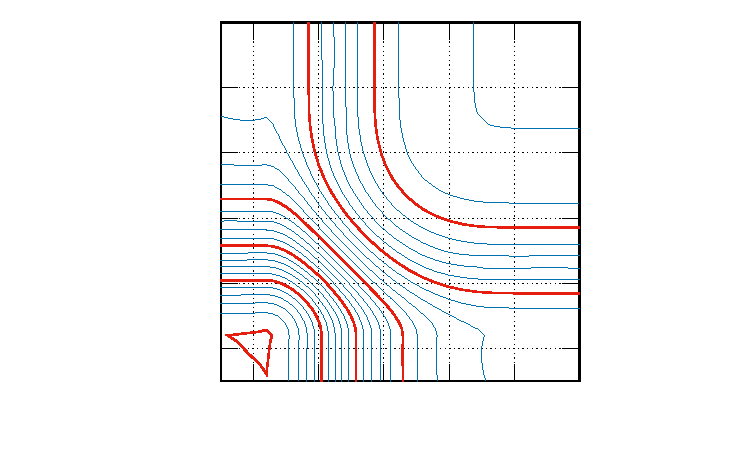
\includegraphics[width={360.00bp},height={216.00bp}]{figmap12zpe}}%
    \gplfronttext
  \end{picture}%
\endgroup
